\documentclass[a4paper,11pt]{refart}
\usepackage{listingsutf8}
\usepackage[utf8]{inputenc}
\usepackage[T1]{fontenc} % LY1 also works
\usepackage{tikz}
\usetikzlibrary{shapes,arrows}
%% Font settings suggested by fbb documentatio
\usepackage{float} 
\usepackage{listings}
\usepackage{microtype}
\usepackage{graphicx}
\usepackage{enumitem}
\setlist{leftmargin=*}
\lstset{basicstyle=\ttfamily,frame=single,xleftmargin=1em,xrightmargin=1em}
\usepackage[os=win]{menukeys}
\renewmenumacro{\keys}[+]{shadowedroundedkeys}
\usepackage{framed}
\usepackage{etoolbox}
\AtBeginEnvironment{leftbar}{\sffamily\small}
\usepackage[T1]{fontenc}
\usepackage{lmodern}
\usepackage{hyperref}
\usepackage{multirow}                                               
\usepackage{multicol}                                               
\usepackage{longtable}
\usepackage{amsmath}
\usepackage{dcolumn}
\usepackage{booktabs}
\usepackage{makecell}

\hypersetup{colorlinks=true,linkcolor=black,citecolor=blue,urlcolor=blue}


\renewcommand\theadalign{bc}
\renewcommand\theadfont{\bfseries}
\renewcommand\theadgape{\Gape[4pt]}
\renewcommand\cellgape{\Gape[4pt]}


\renewcommand\abstractname{Introduction}
\def\CS#1{\texttt{\textbackslash#1}}

\usepackage[most]{tcolorbox}
\newtcblisting{commandshell}{colback=black,colupper=green,colframe=black!75!black,
	listing only,listing options={style=tcblatex,language=sh},
	every listing line={\textcolor{red}{\small\ttfamily\bfseries computer@user:\$ }}}

\usepackage[most]{tcolorbox}
\newtcblisting{shell}{colback=black,colupper=green,colframe=black!75!black,
	listing only,listing options={style=tcblatex,language=sh},
	every listing line={\textcolor{red}{\small\ttfamily\bfseries  }}}


\title{PRIMoRDiA 1.0v Tutorials}
\author{Igor Barden Grillo \\(\url{barden.igor@gmail.com} )\\\url{github.com/igorChem}}

\begin{document}
	\maketitle
	
\begin{abstract}
	PRIMoRDiA ( \textbf{PRI}MoRDiA \textbf{M}acromolecular \textbf{R}eactivity \textbf{D}escriptors \textbf{A}ccess ) is a shared memory parallel software written in C++ for post electronic structure calculations, that efficiently read output files from most used quantum mechanics packages, storing molecular information and processing it to generate several descriptors to evaluate the global and local reactivity of molecular systems. PRIMoRDiA supports the main reactivity descriptors of the Conceptual Density Functional Theory, the most famous and used reactivity theory, which work from response variables of the electronic structure of the molecules, as also other electrostatics properties.
\end{abstract}
\newpage
\section*{Aknowlodgements}

We gratefully thanks the Brazilian science/education institutes by the physical structure and financial support: INCT-INAMI, CNPq,CAPES,FAPESQ-PB, PRONEX-FACEPE and FINEP. Universidade Federal da Paraíba (UFPB) and the computer resources of Centro Nacional de Processamento de Alto Desempenho em São Paulo (CENAPAD-SP). 		
Research project Bioinformática Estrutural de Proteínas: Modelos, Algoritmos e Aplicações Biotecnológicas (Edital Biologia Computacional 51/2013, processo AUXPE1375/2014 da CAPES). G.B.R. acknowledges support from the Brazilian National Council for Scientific and Technological Development (CNPq grant no. 309761/2017-4).

\section{Tutorials}

To learn how to use the program, its features and the auxiliary scripts, you can clone the repository from git hub with the following command

\hspace*{-\leftmarginwidth}
\begin{minipage}{\fullwidth}
	\begin{commandshell}git clone https://github.com/igorChem/PRIMoRDiA1.0v.git\end{commandshell}
\end{minipage}

Or paste this address in your web browser and download the zipped folder.

This repository contains output files for several quantum mechanical calculations needed to get the reactivity descriptors and input files examples for PRIMoRDiA. Also, this is the repository where you have access to the executable and this present document. In this section will be explore the results of PRIMoRDiA from these files.

\subsection{Tutorial 1: Frozen Orbital Examples }

The Frozen Orbital Approximation (FOA) is a calculation method for the global and local descriptors that approximates some of the Conceptual Density Functional Theory derivatives using properties retrieved from the frontier molecular orbitals. Specifically, these molecular orbitals are the Highest energy Occupied Molecular Orbital (HOMO) and the Lowest energy Unoccupied Molecular Orbital (LUMO). To calculate some of the main global descriptors, such as electronic chemical potential and global hardness, the energies values of these molecular orbitals are used. The same is done for the Fukui functions, that are local reactivity descriptors, indicating regioselectivity, and used the spatial distribution of the probability density described by these orbitals.

This approximation method is interesting because requires only one single point calculation for the system studies. Also, brings the relationship with the resolved electronic structure of the system with its chemical reactivity. For more information about these calculation method, its limitations and mathematical development, read the userguide.

\subsubsection{Required Data} 

The required files to run this tutorial are in the data\_test/tutorials/tutorial\_1 folder of the repository. 
The files are of type and extensions of output files from quantum chemistry packages, and a input file of the program. 
This input file can be generated using the option provided along with the program to produce a input files from the names of files in the current folder of a certain quantum chemistry package. \footnote{Tip: Put the PRIMoRDiA executable in .bashrc file with the following command: echo "alias primordia='/path/to/executable/PRIMoRDiA\_1.0v'" >> /home/user/.bashrc }

\hspace*{-\leftmarginwidth}
\begin{minipage}{\fullwidth}
	\begin{commandshell}\end{commandshell}
\end{minipage}

\subsubsection{Creating and Running the input}


\subsubsection{Result Analysis}


\subsection{Tutorial 2: Finite Differences Examples }


\subsection{Tutorial 3: Band Reactivity Descriptors Examples }


\subsection{Tutorial 4: Cube File Generation and Other Options }

If you want generate total electron density or molecular orbitals cube files for the QM programs supported you can use the \emph{"-ed"} or \emph{"-mo"} flags respectively, as will be shown in the following examples. For small molecules, this files can be generated and visualized in common computational chemistry packages, such as Gabedit and Avogradro. Although, these software struggles very often for these tasks for molecules with more than one hundred atoms, then you can use PRIMoRDiA to generate the cube files. 

The first example takes a Gaussian output for the acrolein molecule. In the folder where are the downloaded example files run the following command \footnote{Tip: Put the PRIMoRDiA executable in .bashrc file with the following command: echo "alias primordia='/path/to/executable/PRIMoRDiA\_1.0v'" >> /home/user/.bashrc }to generate the total electron density grid with 40x40x40 of granularity 

\hspace*{-\leftmarginwidth}
\begin{minipage}{\fullwidth}
	\begin{commandshell}primordia -ed acrloein_gauss.fchk 40 gaussian\end{commandshell}
\end{minipage}

The resulted file must have the \emph{"acrloein\_gauss.cube"} name. 
You can open it in pymol software invoking the command\footnote{Tip: Install Pymol software from the linux command line. Try in command line: sudo apt install pymol}

\hspace*{-\leftmarginwidth}
\begin{minipage}{\fullwidth}
	\begin{commandshell}pymol acrloein_gauss.cube\end{commandshell}
\end{minipage}

\begin{figure}[H]
	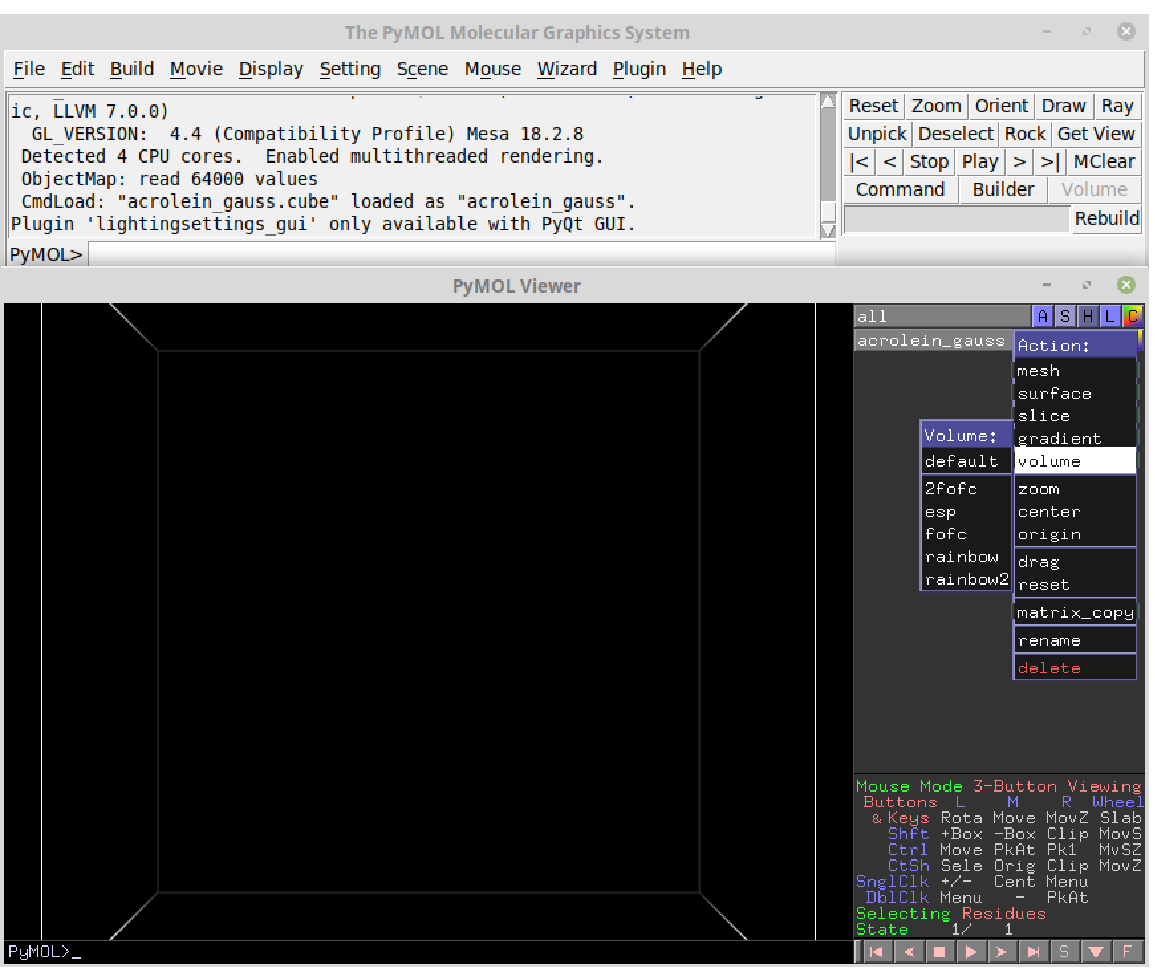
\includegraphics[width=5in]{images_material/figure1}
	\caption{Pymol software window showing the right side bar with volume rendering options.}
	\label{fig1}
\end{figure}

The Pymol window will open with the cube file loaded. To show the iso-surfaces go to the action options in the right side bar and click in \emph{"volume"} and \emph{"default"}, as showed in \autoref{fig1}. To save the image, write in the Pymol terminal emulator   \emph{"draw 800,600"} to render a 800X600 pixel images and \emph{"png acrolein\_gaus.png"} to save in png format, that is shown in \autoref{fig2}. This set of instructions can be followed to generate the images from volume rendering in Pymol in the next tutorial steps. 

\begin{figure}[H]
	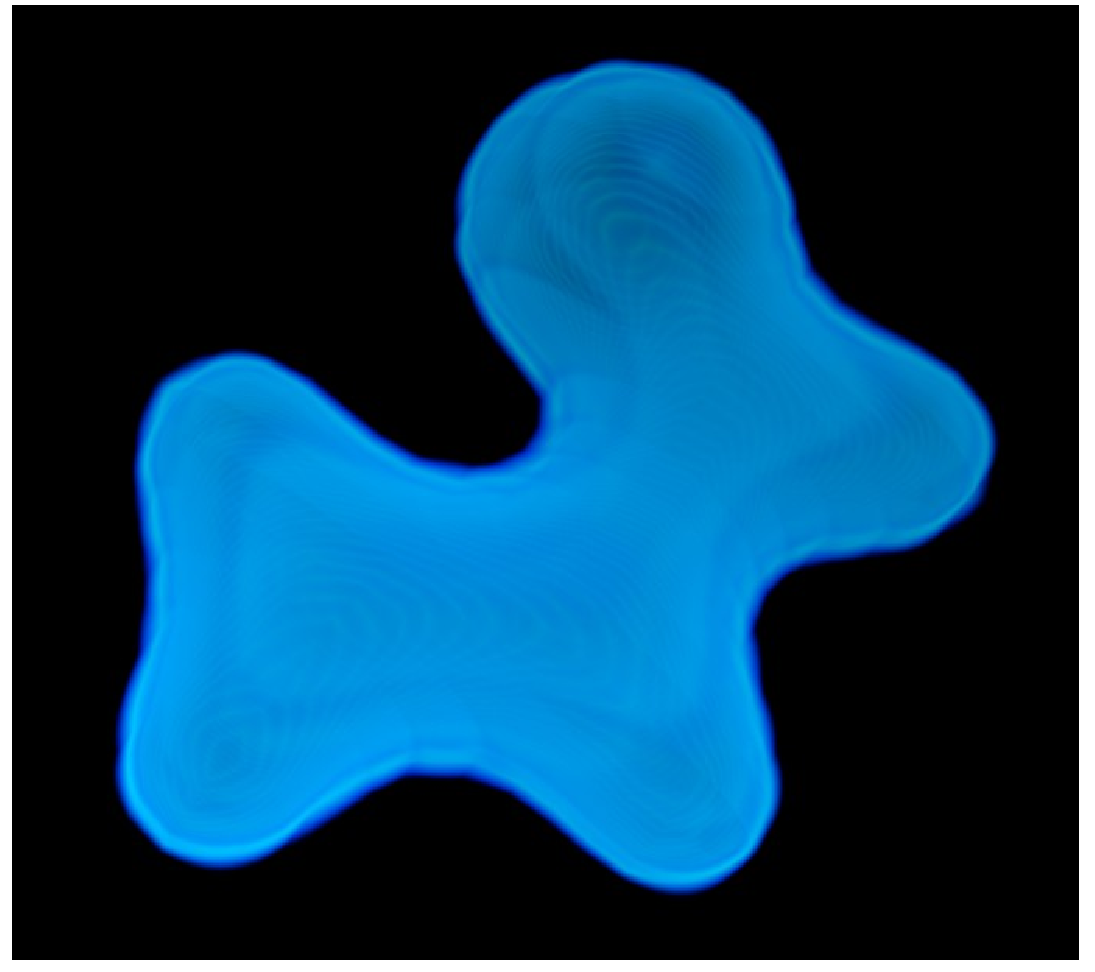
\includegraphics[width=4in]{images_material/figure2}
	\caption{Acrolein total electron density calculated by PRIMoRDiA and saved from Pymol }
	\label{fig2}
\end{figure} 

The generation of Molecular Orbitals 


\hspace*{-\leftmarginwidth}
\begin{minipage}{\fullwidth}
	\begin{commandshell}primordia -mo acrloein_gauss.fchk  40 gaussian\end{commandshell}
\end{minipage}


\subsection{Tutorial 5: Chemical Reaction Analysis with PRIMoRDiA }


\subsection{Tutorial 6: Enzyme Reactivity }


\section{Dealing with Errors}




\end{document}